\documentclass[dvisvgm,border=2pt]{standalone}
% Shared by every figure. Two colours only: black becomes the text colour of
% whatever theme the app is in, and `accent` becomes the brand — see
% scripts/build-figures.mjs. Everything else is done with opacity.
\usepackage{amsmath}
\usepackage{amssymb}
\usepackage{tikz}
\usepackage{pgfplots}
\pgfplotsset{compat=1.18}
\usetikzlibrary{arrows.meta,positioning,calc,backgrounds,fit,patterns.meta}
\definecolor{accent}{RGB}{255,0,255}
\pgfplotsset{
  every axis/.append style={
    axis lines=left,
    axis line style={draw opacity=0.35},
    tick style={draw opacity=0.35},
    tick label style={font=\scriptsize,opacity=0.7},
    label style={font=\scriptsize,opacity=0.7},
    legend style={draw=none,fill=none,font=\scriptsize},
    every axis plot/.append style={line width=0.7pt},
  },
}
\tikzset{
  every picture/.style={font=\scriptsize},
  faint/.style={opacity=0.3},
  quiet/.style={opacity=0.55},
  box/.style={draw,opacity=0.35,rounded corners=2pt,inner sep=4pt},
  hot/.style={accent},
}

\begin{document}
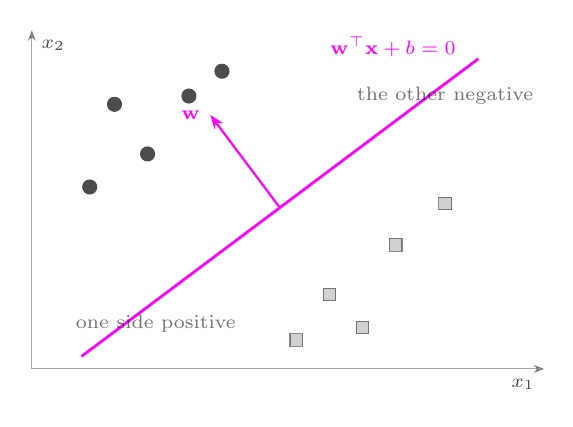
\begin{tikzpicture}[scale=1.05]
  \draw[opacity=0.35,-{Stealth[length=4pt]}] (0,0) -- (6.2,0) node[below left,opacity=0.7]{$x_1$};
  \draw[opacity=0.35,-{Stealth[length=4pt]}] (0,0) -- (0,4.1) node[below right,opacity=0.7]{$x_2$};
  % the boundary
  \draw[accent,line width=1pt] (0.6,0.15) -- (5.4,3.75)
    node[above left,accent,pos=0.97]{$\mathbf{w}^{\top}\mathbf{x}+b=0$};
  % its normal
  \draw[accent,-{Stealth[length=5pt]},line width=0.8pt] (3,1.95) -- (2.16,3.07)
    node[left,accent]{$\mathbf{w}$};
  \foreach \p in {(1.4,2.6),(1.0,3.2),(1.9,3.3),(0.7,2.2),(2.3,3.6)}
    \fill[opacity=0.7] \p circle (2.6pt);
  \foreach \p in {(3.6,0.9),(4.4,1.5),(4.0,0.5),(5.0,2.0),(3.2,0.35)}
    \draw[opacity=0.45,fill,fill opacity=0.18] \p ++(-2.2pt,-2.2pt) rectangle ++(4.4pt,4.4pt);
  \node[opacity=0.55,align=left] at (1.5,0.55) {one side\ positive};
  \node[opacity=0.55,align=left] at (5.0,3.3) {the other\ negative};
\end{tikzpicture}
\end{document}
